% vim: set fdm=marker:
\pdfminorversion=4
\documentclass[mathserif]{beamer}

% theme {{{
%\usetheme{Antibes}
\usetheme[compress]{Dresden}
%\usecolortheme{dolphin}
\usecolortheme{rose}
%\usefonttheme{serif}
%}}}

% packages {{{
\usepackage[english]{babel}
\usepackage[utf8]{inputenc}
\usepackage[T1]{fontenc}
\usepackage{caption}
\usepackage{tikz}
%}}}

% config {{{
\colorlet{lightbg}{yellow!20}
\colorlet{lightborder}{yellow!50!black}
\colorlet{graybg}{black!10}
\colorlet{grayborder}{black!50}

\usetikzlibrary{fit,positioning,chains,scopes,shapes,shapes.multipart,calc}

\tikzset{
	node grid/.style={row sep=1ex, column sep=1.5ex},
	small node/.style={very thick, text height=1ex, text depth=.25ex, rounded corners, node distance=1.5ex},
    split node/.style={rectangle split, rectangle split parts=#1},
	document node/.style={small node, draw=lightborder, fill=lightbg},
	operation node/.style={small node, draw=grayborder, fill=graybg},
	connector/.style={very thick, draw=grayborder, ->, rounded corners},
	vh connector/.style={connector, to path={|- (\tikztotarget)}},
	hv connector/.style={connector, to path={-| (\tikztotarget)}},
    hvh connector top/.style={to path={-- ++(1.5ex,0) |- (\tikztotarget.170)}},
    hvh connector bottom/.style={to path={-- ++(1.5ex,0) |- (\tikztotarget.190)}},
    left offset/.style={right=1.5ex}
}

\usepackage{pgfplots}
\usepackage{pgfplotstable}
\usepackage{multirow}
\usepackage{booktabs}


%\pgfplotstableset{col sep=comma}
\pgfplotsset{
    /pgfplots/flexible yticklabels from table/.code n args={2}{%
        \pgfplotstablegetcolumn{#2}\of{#1}\to\pgfplots@yticklabels
        \let\pgfplots@yticklabel=\pgfplots@user@ticklabel@list@y
    },
    hbarplot/.style={
        xbar,
        small,
        y=-\baselineskip,
        enlarge y limits={true, abs value=0.45},
        xmin=0,
        xmax=0.3,
        ytick=\empty,
        xticklabel style={/pgf/number format/.cd,fixed,precision=2},
        nodes near coords,
        nodes near coords align=horizontal,
        every node near coord/.append style={font=\tiny, /pgf/number format/.cd,fixed,precision=3},
        axis x line*=bottom,
        axis y line*=left,
    }
    }

\pgfplotstableset{create on use/graph/.style={
create col/expr=0
}}
\pgfplotstableread[]{results/reference.csv}\resultsreference
\newcommand{\addreferenceplot}{\addplot[const plot, red, update limits=false] table[x=MeanCorrelation, y expr=\coordindex*100-1] {\resultsreference}}

\newcommand{\plotxbars}[1]{%
    \begin{tikzpicture}
        \begin{axis}[
            hbarplot,
            width=6cm,
            ]
            \addplot table[x=MeanCorrelation, y expr=\coordindex] {#1};
            \addreferenceplot;
        \end{axis}
    \end{tikzpicture}%
}

\newcommand{\plottablexbars}[2]{
    \pgfplotstablegetrowsof{#2}
    \let\numberofrows=\pgfplotsretval

    \pgfplotstabletypeset[columns={#1,graph},
      % Booktabs rules
      every head row/.style={after row=\midrule},
      every last row/.style={after row=[3ex]},
      % Set header name
      columns/scales/.style={string type,column name=$N_s$},
      columns/angles/.style={string type,column name=$N_{\theta}$},
      columns/gridsize/.style={string type,column name=$G$},
      columns/patchsize/.style={string type,column name=$P$},
      columns/cannysigma/.style={string type,column name=$\sigma$},
      columns/metric/.style={string type,column name=Metric},
      columns/graph/.style={
        column name={},
        assign cell content/.code={% use \multirow for Z column:
        \ifnum\pgfplotstablerow=0
        \pgfkeyssetvalue{/pgfplots/table/@cell content}
        {\multirow{\numberofrows}{5cm}{\plotxbars{#2}}}%
        \else
        \pgfkeyssetvalue{/pgfplots/table/@cell content}{}%
        \fi
        }
      },
    ]{#2}
}

%\captionsetup{font=scriptsize,labelfont=scriptsize}
%\renewcommand{\captionfont}{\tiny}
%\renewcommand{\captionlabelfont}{\tiny}
%\setlength{\intextsep}{5.0pt plus 2.0pt minus 2.0pt}
%}}}

% title {{{
\title{Analysis of Image Tranforms for Sketch-based Retrieval}
\subtitle{Diploma Thesis}
\author{Felix Stürmer}
\institute[Fakultät IV - TU Berlin]
{
    Technische Universität Berlin\\
    Fakultät IV - Elektrotechnik und Informatik\\
    Computer Graphics
}
\date{02.11.2012}
\subject{Computer Graphics}
%}}}

\begin{document}
% document {{{

% titlepage {{{
\begin{frame}
  \titlepage
\end{frame}
%}}}

% toc {{{
\begin{frame}{Outline}
  \tableofcontents
  % You might wish to add the option [pausesections]
\end{frame}
%}}}

% introduction and background {{{
\section{Introduction and Background}
\subsection{Motivation and Challenges of CBIR}
\begin{frame}{Motivation}
    foo
\end{frame}

\begin{frame}{Challenges of CBIR}
    \begin{block}{The Semantic Gap}
        \begin{quote}
            ``The semantic gap is the \textbf{lack of coincidence} between the
            information that one can extract from the \textbf{visual data} and
            the \textbf{interpretation} that the same data have for a user in a
            given situation.'' -- Smeulders et al.
        \end{quote}
    \end{block}
    \begin{block}{The Sensory Gap}
        \begin{quote}
            ``The sensory gap is the gap between the \textbf{object in the
            world} and the information in a (computational) description derived
            from a \textbf{recording of that scene}.'' -- Smeulders et al.
        \end{quote}
    \end{block}
\end{frame}

\subsection{Prior Work}
\begin{frame}{Prior Work on Human Recognition}
    \begin{figure}
        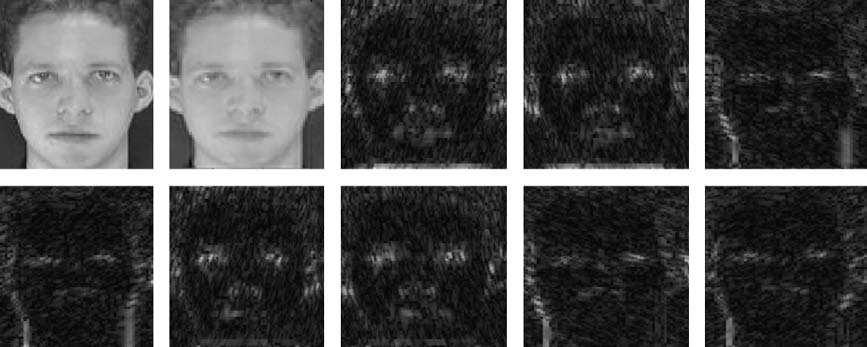
\includegraphics[width=.9\textwidth]{illustrations/related_work/curvelet_faces_mandal09}
        \caption{``Face recognition using curvelet based PCA.'', T. Mandal and Q. M.J Wu, ICPR 2008}
    \end{figure}
\end{frame}

\begin{frame}{Prior Work on Human Recognition}
    \begin{figure}
        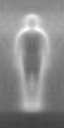
\includegraphics[width=.12\textwidth]{illustrations/related_work/hog_dalal05_1}
        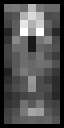
\includegraphics[width=.12\textwidth]{illustrations/related_work/hog_dalal05_2}
        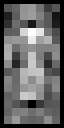
\includegraphics[width=.12\textwidth]{illustrations/related_work/hog_dalal05_3}
        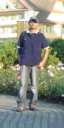
\includegraphics[width=.12\textwidth]{illustrations/related_work/hog_dalal05_4}
        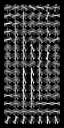
\includegraphics[width=.12\textwidth]{illustrations/related_work/hog_dalal05_5}
        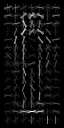
\includegraphics[width=.12\textwidth]{illustrations/related_work/hog_dalal05_6}
        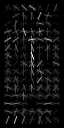
\includegraphics[width=.12\textwidth]{illustrations/related_work/hog_dalal05_7}
        \caption{``Histograms of oriented gradients for human detection'', Dalal and Triggs, CVPR 2005}
    \end{figure}
\end{frame}

\begin{frame}{Prior Work on Visual Codebooks}
    \begin{columns}
        \begin{column}{.5\textwidth}
            \begin{figure}
                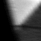
\includegraphics[width=.5cm]{illustrations/related_work/video_google/video_google_dict1_1}
                
\includegraphics[width=.5cm]{illustrations/related_work/video_google/video_google_dict1_2}
                
\includegraphics[width=.5cm]{illustrations/related_work/video_google/video_google_dict1_3}
                
\includegraphics[width=.5cm]{illustrations/related_work/video_google/video_google_dict1_4}
                
\includegraphics[width=.5cm]{illustrations/related_work/video_google/video_google_dict1_5}
                
\includegraphics[width=.5cm]{illustrations/related_work/video_google/video_google_dict1_6}\\
                
\includegraphics[width=.5cm]{illustrations/related_work/video_google/video_google_dict1_7}
                
\includegraphics[width=.5cm]{illustrations/related_work/video_google/video_google_dict1_8}
                
\includegraphics[width=.5cm]{illustrations/related_work/video_google/video_google_dict1_9}
                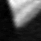
\includegraphics[width=.5cm]{illustrations/related_work/video_google/video_google_dict1_10}
                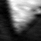
\includegraphics[width=.5cm]{illustrations/related_work/video_google/video_google_dict1_11}
                
\includegraphics[width=.5cm]{illustrations/related_work/video_google/video_google_dict1_12}\\
                
\includegraphics[width=.5cm]{illustrations/related_work/video_google/video_google_dict1_13}
                
\includegraphics[width=.5cm]{illustrations/related_work/video_google/video_google_dict1_14}
                
\includegraphics[width=.5cm]{illustrations/related_work/video_google/video_google_dict1_15}
                
\includegraphics[width=.5cm]{illustrations/related_work/video_google/video_google_dict1_16}
                
\includegraphics[width=.5cm]{illustrations/related_work/video_google/video_google_dict1_17}
                
\includegraphics[width=.5cm]{illustrations/related_work/video_google/video_google_dict1_18}\\
                
\includegraphics[width=.5cm]{illustrations/related_work/video_google/video_google_dict1_19}
                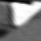
\includegraphics[width=.5cm]{illustrations/related_work/video_google/video_google_dict1_20}
                
\includegraphics[width=.5cm]{illustrations/related_work/video_google/video_google_dict1_21}
                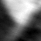
\includegraphics[width=.5cm]{illustrations/related_work/video_google/video_google_dict1_22}
                
\includegraphics[width=.5cm]{illustrations/related_work/video_google/video_google_dict1_23}
                
\includegraphics[width=.5cm]{illustrations/related_work/video_google/video_google_dict1_24}\\
                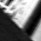
\includegraphics[width=.5cm]{illustrations/related_work/video_google/video_google_dict1_25}
                
\includegraphics[width=.5cm]{illustrations/related_work/video_google/video_google_dict1_26}
                
\includegraphics[width=.5cm]{illustrations/related_work/video_google/video_google_dict1_27}
                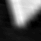
\includegraphics[width=.5cm]{illustrations/related_work/video_google/video_google_dict1_28}
                
\includegraphics[width=.5cm]{illustrations/related_work/video_google/video_google_dict1_29}
                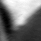
\includegraphics[width=.5cm]{illustrations/related_work/video_google/video_google_dict1_30}
            \end{figure}
            \begin{figure}
                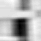
\includegraphics[width=.5cm]{illustrations/related_work/video_google/video_google_dict2_1}
                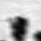
\includegraphics[width=.5cm]{illustrations/related_work/video_google/video_google_dict2_2}
                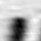
\includegraphics[width=.5cm]{illustrations/related_work/video_google/video_google_dict2_3}
                
\includegraphics[width=.5cm]{illustrations/related_work/video_google/video_google_dict2_4}
                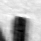
\includegraphics[width=.5cm]{illustrations/related_work/video_google/video_google_dict2_5}
                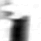
\includegraphics[width=.5cm]{illustrations/related_work/video_google/video_google_dict2_6}\\
                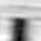
\includegraphics[width=.5cm]{illustrations/related_work/video_google/video_google_dict2_7}
                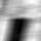
\includegraphics[width=.5cm]{illustrations/related_work/video_google/video_google_dict2_8}
                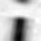
\includegraphics[width=.5cm]{illustrations/related_work/video_google/video_google_dict2_9}
                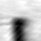
\includegraphics[width=.5cm]{illustrations/related_work/video_google/video_google_dict2_10}
                
\includegraphics[width=.5cm]{illustrations/related_work/video_google/video_google_dict2_11}
                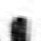
\includegraphics[width=.5cm]{illustrations/related_work/video_google/video_google_dict2_12}\\
                \includegraphics[width=.5cm]{illustrations/related_work/video_google/video_google_dict2_13}
                \includegraphics[width=.5cm]{illustrations/related_work/video_google/video_google_dict2_14}
                \includegraphics[width=.5cm]{illustrations/related_work/video_google/video_google_dict2_15}
                \includegraphics[width=.5cm]{illustrations/related_work/video_google/video_google_dict2_16}
                \includegraphics[width=.5cm]{illustrations/related_work/video_google/video_google_dict2_17}
                \includegraphics[width=.5cm]{illustrations/related_work/video_google/video_google_dict2_18}\\
                \includegraphics[width=.5cm]{illustrations/related_work/video_google/video_google_dict2_19}
                \includegraphics[width=.5cm]{illustrations/related_work/video_google/video_google_dict2_20}
                \includegraphics[width=.5cm]{illustrations/related_work/video_google/video_google_dict2_21}
                \includegraphics[width=.5cm]{illustrations/related_work/video_google/video_google_dict2_22}
                \includegraphics[width=.5cm]{illustrations/related_work/video_google/video_google_dict2_23}
                \includegraphics[width=.5cm]{illustrations/related_work/video_google/video_google_dict2_24}\\
                \includegraphics[width=.5cm]{illustrations/related_work/video_google/video_google_dict2_25}
                \includegraphics[width=.5cm]{illustrations/related_work/video_google/video_google_dict2_26}
                \includegraphics[width=.5cm]{illustrations/related_work/video_google/video_google_dict2_27}
                \includegraphics[width=.5cm]{illustrations/related_work/video_google/video_google_dict2_28}
                \includegraphics[width=.5cm]{illustrations/related_work/video_google/video_google_dict2_29}
                \includegraphics[width=.5cm]{illustrations/related_work/video_google/video_google_dict2_30}
            \end{figure}
        \end{column}
        \begin{column}{.5\textwidth}
            \begin{figure}
                \includegraphics[width=.4\textwidth]{illustrations/related_work/video_google/query_1_large}
                \includegraphics[width=.4\textwidth]{illustrations/related_work/video_google/query_1_small}\\
                \includegraphics[width=.4\textwidth]{illustrations/related_work/video_google/query_2_large}
                \includegraphics[width=.4\textwidth]{illustrations/related_work/video_google/query_2_small}
                \caption{``Video Google: A text retrieval approach to object matching in videos'', Sivic and Zisserman, ICCV 2003}
            \end{figure}
        \end{column}
    \end{columns}
\end{frame}

\begin{frame}{Prior Work on Scene Classification}
    \begin{figure}
        \includegraphics[width=.9\textwidth]{illustrations/related_work/pyramid_lazebnik09}
        \caption{``Spatial pyramid matching'', Lazebnik et al., 2009}
    \end{figure}
\end{frame}

\subsection{Anatomy of a CBIR System}
\begin{frame}{Anatomy of a CBIR System}
    \begin{columns}
        \begin{column}{0.5\textwidth}
            \begin{figure}
                \includegraphics[width=.9\textwidth]{illustrations/cbir_anatomy_query_cropped}
                \caption{Global Descriptors}
                \label{fig:anatomy_global}
            \end{figure}
        \end{column}
        \begin{column}{0.5\textwidth}
            \begin{figure}
                \includegraphics[width=.9\textwidth]{illustrations/cbir_anatomy_query_local_cropped}
                \caption{Local Descriptors}
                \label{fig:anatomy_local}
            \end{figure}
        \end{column}
    \end{columns}
\end{frame}
% }}}

% solution {{{
\section{Proposed Solution}
\subsection{Proposed Retrieval Pipelines}
\begin{frame}{Proposed Retrieval Pipelines (Global)}
    \begin{figure}
        %\begin{tikzpicture}[font=\tiny]
    \matrix[node grid] {
        \node [document node] (dbimg) {$I_{db}$}; &
        \node [operation node, split node=4] (dbpreprocess) {LUMA \nodepart{two} LUMA+SOBEL \nodepart{three} LUMA+CANNY \nodepart{four} SEGMENT};  &
        \node [operation node] (dbcurvelet) {FDCT}; &
        \node [operation node] (dbmean) {MEAN}; \\
        \node [document node] (qimg) {$I_q$}; &
        \node [operation node] (qluma) {LUMA}; &
        \node [operation node] (qcurvelet) {FDCT}; &
        \node [operation node] (qmean) {MEAN}; \\
    };

    \node [operation node, split node=2, right=3ex of $(dbmean.east)!0.5!(qmean.east)$] (dist) {$L_2$ \nodepart{two} COS};
    \node [document node, right=of dist] (result) {distances};

    \node [parameter node, below=1ex of dbimg] (dbcannyparam) {$\sigma$};
    \node [parameter node, above=of dbcurvelet] (dbcurveletparam) {$(N_s, N_{\theta})$};
    \node [parameter node, above=of dbmean] (dbmeanparam) {$G$};
    \node [parameter node, below=of qcurvelet] (qcurveletparam) {$(N_s, N_{\theta})$};
    \node [parameter node, below=of qmean] (qmeanparam) {$G$};

    \path [parameter connector] (dbcannyparam) -- (dbpreprocess.three west);
    \path [parameter connector] (dbcurveletparam) -- (dbcurvelet);
    \path [parameter connector] (dbmeanparam) -- (dbmean);
    \path [parameter connector] (qcurveletparam) -- (qcurvelet);
    \path [parameter connector] (qmeanparam) -- (qmean);

    { [start chain=going right, every join/.style={connector}]
        \chainin (dbimg);
        \chainin (dbpreprocess) [join];
        \chainin (dbcurvelet) [join];
        \chainin (dbmean) [join];
        \chainin (dist) [join=with dbmean.east by hvh connector top];
    }
    { [start chain=going right, every join/.style={connector}]
        \chainin (qimg);
        \chainin (qluma) [join];
        \chainin (qcurvelet) [join];
        \chainin (qmean) [join];
        \chainin (dist) [join=with qmean.east by hvh connector bottom];
        \chainin (result) [join];
    }

    \begin{pgfonlayer}{background}
        \node[minimum node, above=of dbimg] (labelanchor) {};
        \node[minimum node, below=of qimg] (labelanchorbottom) {};
        \node (acquisitionend) at ($(dbpreprocess.east)!0.5!(dbcurvelet.west)$) {};
        \node (extractionmiddle) at ($(dbcurvelet.east)!0.5!(dbmean.west)$) {};
        \node (extractionend) at ($(dbmean.east)!0.5!(dist.west)$) {};
        \node (rankingmiddle) at ($(dist.east)!0.5!(result.west)$) {};

        \only<2>{\path[section highlight] (labelanchor.north west) rectangle (labelanchorbottom.south -| acquisitionend);}
        \only<3>{\path[section highlight] (labelanchor.north west -| acquisitionend) rectangle (labelanchorbottom.south -| extractionend);}
        \only<4>{\path[section highlight] (labelanchor.north west -| extractionend) rectangle (labelanchorbottom.south -| result.east);}

        \node[section label] (acquisitionlabel) at (labelanchor -| dbpreprocess) {Acquisition};
        \node[section label] (extractionlabel) at (labelanchor -| extractionmiddle) {Feature Extraction};
        \node[section label] (rankinglabel) at (labelanchor -| rankingmiddle) {Ranking};
        \path[section divider] (labelanchor.north -| acquisitionend) -- (labelanchorbottom.south -| acquisitionend);
        \path[section divider] (labelanchor.north -| extractionend) -- (labelanchorbottom.south -| extractionend);
    \end{pgfonlayer}
\end{tikzpicture}

    \end{figure}
\end{frame}

\begin{frame}{Proposed Retrieval Pipelines (Local)}
    \begin{figure}
        %\begin{tikzpicture}[font=\tiny]
    \matrix[node grid] {
        \node [document node] (dbimg) {$I_{db}$}; &
        \node [operation node, split node=4] (dbpreprocess) {LUMA \nodepart{two} LUMA+SOBEL \nodepart{three} LUMA+CANNY \nodepart{four} SEGMENT};  &
        \node [operation node] (dbcurvelet) {FDCT}; &
        %\node [operation node] (dbpmean) {PMEAN}; &&
        \node [operation node, split node=2] (dbpmean) {PMEAN \nodepart{two} PMEAN2}; &
        \node [operation node] (dbquant) {VQ}; \\
        &&&
        \node [operation node] (cluster) {CLUSTER}; \\
        \node [document node] (qimg) {$I_q$}; &
        \node [operation node] (qluma) {LUMA}; &
        \node [operation node] (qcurvelet) {FDCT}; &
        %\node [operation node] (qpmean) {PMEAN}; &&
        \node [operation node, split node=2] (qpmean) {PMEAN \nodepart{two} PMEAN2}; &
        \node [operation node] (qquant) {VQ}; \\
    };
    \node [operation node, split node=4, right=3ex of $(dbquant.east)!0.5!(qquant.east)$] (dist) {$L_2$ \nodepart{two} COS \nodepart{three} HI(B) \nodepart{four} EMD};
    \node [document node, right=of dist] (result) {distances};

    \node [parameter node, below=1ex of dbimg] (dbcannyparam) {$\sigma$};
    \node [parameter node, above=of dbcurvelet] (dbcurveletparam) {$(N_s, N_{\theta})$};
    \node [parameter node, above=of dbpmean] (dbpmeanparam) {$(G, P)$};
    \node [parameter node, below=of qcurvelet] (qcurveletparam) {$(N_s, N_{\theta})$};
    \node [parameter node, below=of qpmean] (qpmeanparam) {$(G, P)$};

    \path [parameter connector] (dbcannyparam) -- (dbpreprocess.three west);
    \path [parameter connector] (dbcurveletparam) -- (dbcurvelet);
    \path [parameter connector] (dbpmeanparam) -- (dbpmean);
    \path [parameter connector] (qcurveletparam) -- (qcurvelet);
    \path [parameter connector] (qpmeanparam) -- (qpmean);

    { [start chain=going right, every join/.style={connector}]
        \chainin (dbimg);
        \chainin (dbpreprocess) [join];
        \chainin (dbcurvelet) [join];
        \chainin (dbpmean) [join];
        { [start branch]
            \chainin (cluster) [join];
            { [start branch]
                \chainin (qquant) [join=with cluster.-5 by hv connector];
            }
            \chainin (dbquant) [join=with cluster.5 by hv connector];
        }
        \chainin (dbquant) [join];
        \chainin (dist) [join=with dbquant.east by hvh connector top];
    }
    { [start chain=going right, every join/.style={connector}]
        \chainin (qimg);
        \chainin (qluma) [join];
        \chainin (qcurvelet) [join];
        \chainin (qpmean) [join];
        \chainin (qquant) [join];
        \chainin (dist) [join=with qquant.east by hvh connector bottom];
        \chainin (result) [join];
    }

    \begin{pgfonlayer}{background}
        \node[minimum node, above=of dbimg] (labelanchor) {};
        \node[minimum node, below=of qimg] (labelanchorbottom) {};
        \node (acquisitionend) at ($(dbpreprocess.east)!0.5!(dbcurvelet.west)$) {};
        \node (extractionmiddle) at ($(dbcurvelet.east)!0.5!(dbquant.west)$) {};
        \node (extractionend) at ($(dbquant.east)!0.5!(dist.west)$) {};
        \node (rankingmiddle) at ($(dist.east)!0.5!(result.west)$) {};

        \only<2>{\path[section highlight] (labelanchor.north west) rectangle (labelanchorbottom.south -| acquisitionend);}
        \only<3>{\path[section highlight] (labelanchor.north west -| acquisitionend) rectangle (labelanchorbottom -| extractionend);}
        \only<4>{\path[section highlight] (labelanchor.north west -| extractionend) rectangle (labelanchorbottom -| result.east);}

        \node[section label] (acquisitionlabel) at (labelanchor -| dbpreprocess) {Acquisition};
        \node[section label] (extractionlabel) at (labelanchor -| extractionmiddle) {Feature Extraction};
        \node[section label] (rankinglabel) at (labelanchor -| rankingmiddle) {Ranking};
        \path[section divider] (labelanchor.north -| acquisitionend) -- (labelanchorbottom.south -| acquisitionend);
        \path[section divider] (labelanchor.north -| extractionend) -- (labelanchorbottom.south -| extractionend);
    \end{pgfonlayer}
\end{tikzpicture}

    \end{figure}
\end{frame}

\subsection{Acquisition}
\begin{frame}{Acquisition}
    \begin{columns}[T]
        \begin{column}{0.5\textwidth}
            \begin{figure}
                \includegraphics[width=\textwidth]{illustrations/input_example_color}
                \caption{Original Image}
            \end{figure}
        \end{column}
        \begin{column}{0.5\textwidth}
            \only<1>{
                \begin{figure}
                    \includegraphics[width=\textwidth]{illustrations/input_example_luma}
                    \caption{Luma Conversion}
                \end{figure}
            }
            \only<2>{
                \begin{figure}
                    \includegraphics[width=\textwidth]{illustrations/input_example_canny}
                    \caption{Canny Operator}
                \end{figure}
            }
            \only<3>{
                \begin{figure}
                    \includegraphics[width=\textwidth]{illustrations/input_example_sobel}
                    \caption{Sobel Operator}
                \end{figure}
            }
            \only<4>{
                \begin{figure}
                    \includegraphics[width=\textwidth]{illustrations/input_example_segment}
                    \caption{gPb-owt-ucm Transform}
                \end{figure}
            }
        \end{column}
    \end{columns}
\end{frame}

\subsection{The Curvelet Transform}
\begin{frame}{Properties of the Curvelet Transform}
    \begin{itemize}
        \item An extension of the wavelet transform
        \item Localized in \emph{position}, \emph{scale} and \emph{orientation}
        \item Curvelets obey parabolic scaling: $width \approx length^2$
        \item Approximation error along edges using $m$ largest coefficients decays with $\frac{log(m)^3}{m^2}$ (compare $\frac{1}{m}$ for wavelets)
        \item Defined in frequency domain using 
    \end{itemize}
\end{frame}

\begin{frame}{Constructing the Curvelets}
    \begin{columns}
        \begin{column}{.5\textwidth}
            \begin{figure}
                \begin{tikzpicture}[font=\tiny,x=0.75cm,y=0.75cm]
    \def\ra{.05}
    \def\rb{.1}
    \def\rc{.2}
    \def\rd{.4}
    \def\re{.8}
    \def\rf{1.6}
    \def\rg{3.2}
    \coordinate (center) at (0,0);

    % draw shells
    \foreach \r in {\ra,\rb,\rc,\rd,\re,\rf,\rg} {
        \draw[default line] (center) circle(\r);
    }

    % draw angular lines
    \uncover<2->{
        \foreach \a in {0,90,180,270} {
            \draw[default line] (\a:\ra) -- (\a:\rg);
        }
    %}

    %\uncover<3->{
        \foreach \a in {45,135,...,360} {
            \draw[default line] (\a:\rb) -- (\a:\rg);
        }
    %}

    %\uncover<4->{
        \foreach \a in {22.5,67.5,...,360} {
            \draw[default line] (\a:\rd) -- (\a:\rg);
        }
    %}

    %\uncover<5->{
        \foreach \a in {11.25,33.75,...,360} {
            \draw[default line] (\a:\rf) -- (\a:\rg);
        }
    }

    \uncover<4->{
        \draw[highlight line] (center) circle(2.4);
        \node[text=red, anchor=north west] at (0:2.4) {Scale};
        \draw[highlight line] (center) -- (50.75:4);
        \node[text=red, anchor=west] at (50.75:\rg) {Orientation};
    }

    \begin{pgfonlayer}{background}
        \uncover<3->{
            \path[highlight area] (56.25:\rf) -- (56.25:\rg) arc[start angle=56.25, end angle=45, radius=\rg] -- (45:\rf) arc[start angle=45, end angle=56.25, radius=\rf];

            \path[default line, decorate, decoration={brace, mirror}] (45:\rf) to node[below right=-0.15, midway]{$2^j$} (45:\rg);
            \path[default line, decorate, decoration={brace, mirror}] (45:\rg) to node[above right=-0.05, midway]{$2^{\frac{j}{2}}$} (56.25:\rg);
        }
    \end{pgfonlayer}
\end{tikzpicture}

                \caption{Frequency Domain}
            \end{figure}
        \end{column}
        \begin{column}{.5\textwidth}
            \begin{figure}
                \begin{tikzpicture}[font=\tiny,x=0.55cm,y=0.55cm,rotate=-45]
    % draw dots
    \uncover<2->{
        \foreach \x in {3.2,6.4,9.6}
            \foreach \y in {1,...,7} {
                \draw[fill=black] (\x, \y) circle(0.04);
        }
    }

    \uncover<4->{
        \path[highlight line, ->] (6.4, 4) to node[left, midway, text=red]{Translation} (9.6, 2);
    }

    \begin{pgfonlayer}{background}
        \uncover<3->{
            \path[default line, highlight area] (9.6, 2) circle[x radius=1.6, y radius=.5];

            \path[default line, decorate, decoration={brace}] (6.4, 4) to node[above right=-0.05, midway]{$2^{-\frac{j}{2}}$} (9.6, 4);
            \path[default line, decorate, decoration={brace}] (9.6, 4) to node[below right=-0.15, midway]{$2^{-j}$} (9.6, 3);
        }
    \end{pgfonlayer}
\end{tikzpicture}

                \caption{Spatial Domain}
            \end{figure}
        \end{column}
    \end{columns}
\end{frame}

\begin{frame}{Example Curvelets}
    \begin{columns}
        \begin{column}{.5\textwidth}
            \begin{figure}
                \includegraphics[width=.5\textwidth]{illustrations/curvelet_examples/curvelet_1_frequency}\\
                \includegraphics[width=.5\textwidth]{illustrations/curvelet_examples/curvelet_2_frequency}
                \caption{Frequency Domain}
            \end{figure}
        \end{column}
        \begin{column}{.5\textwidth}
            \begin{figure}
                \includegraphics[width=.5\textwidth]{illustrations/curvelet_examples/curvelet_1_time}\\
                \includegraphics[width=.5\textwidth]{illustrations/curvelet_examples/curvelet_2_time}
                \caption{Spatial Domain}
            \end{figure}
        \end{column}
    \end{columns}
\end{frame}

\begin{frame}{The Fast Discrete Curvelet Transform}
    \begin{columns}
        \begin{column}{.5\textwidth}
            \begin{figure}
                \begin{tikzpicture}[font=\tiny,x=0.75cm,y=0.75cm]
    \def\ra{.05}
    \def\rb{.1}
    \def\rc{.2}
    \def\rd{.4}
    \def\re{.8}
    \def\rf{1.6}
    \def\rg{3.2}
    \coordinate (center) at (0,0);
    \def\rectc{(-\rc, -\rc) rectangle (\rc, \rc)}
    \def\rectd{(-\rd, -\rd) rectangle (\rd, \rd)}
    \def\recte{(-\re, -\re) rectangle (\re, \re)}
    \def\rectf{(-\rf, -\rf) rectangle (\rf, \rf)}
    \def\rectg{(-\rg, -\rg) rectangle (\rg, \rg)}

    \coordinate (lvt) at (\re, 4);
    \coordinate (lvb) at (\re, -4);
    \coordinate (rvt) at (\rf, 4);
    \coordinate (rvb) at (\rf, -4);
    \coordinate (thr) at (33.75:10);
    \coordinate (bhr) at (22.5:10);

    \coordinate (wtl) at (intersection of lvt--lvb and center--thr);
    \coordinate (wtr) at (intersection of rvt--rvb and center--thr);
    \coordinate (wbr) at (intersection of rvt--rvb and center--bhr);
    \coordinate (wbl) at (intersection of lvt--lvb and center--bhr);

    \draw[default area] \rectg;
    \begin{scope}
        \clip \rectg;
        \foreach \a in {0,5.625,...,359} {
            \draw[default line] (center) -- (\a:10);
        }
    \end{scope}

    \draw[default area] \rectf;
    \begin{scope}
        \clip \rectf;
        \foreach \a in {0,11.25,...,359} {
            \draw[default line] (center) -- (\a:10);
        }
    \end{scope}

    \draw[default area] \rectf;
    \draw[default area] \recte;
    \begin{scope}
        \clip \rectf;
        \uncover<2->{
            \path[highlight area] (wtl) -- (wtr) -- (wbr) -- (wbl) -- cycle;
        }
        \foreach \a in {0,11.25,...,359} {
            \draw[default line] (center) -- (\a:10);
        }
    \end{scope}
    \draw[default line] \rectf;
    \draw[default line] \recte;

    \draw[default area] \rectd;
    \begin{scope}
        \clip \rectd;
        \foreach \a in {0,22.5,...,359} {
            \draw[default line] (center) -- (\a:10);
        }
    \end{scope}

    \draw[default area] \rectc;


    % draw shells
    %\foreach \r in {\rc,\rd,\re,\rf,\rg} {
        %\draw[default line] (-\r, -\r) rectangle (\r, \r);
    %}

    %\begin{scope}
        %\clip (-\rg, -\rg) rectangle (\rg, \rg);
        %% draw angular lines
        %\foreach \a in {0,90,180,270} {
            %\draw[default line] (\a:\ra) -- (\a:\rg);
        %}

        %%\foreach \a in {45,135,...,360} {
            %%\draw[default line] (\a:\rb) -- (\a:\rg);
        %%}

        %%\foreach \a in {22.5,67.5,...,360} {
            %%\draw[default line] (\a:\rd) -- (\a:\rg);
        %%}

        %%\foreach \a in {11.25,33.75,...,360} {
            %%\draw[default line] (\a:\rf) -- (\a:\rg);
        %%}
    %\end{scope}

    %\uncover<7->{
        %\draw[highlight line] (center) circle(2.4);
        %\node[text=red, anchor=north west] at (0:2.4) {Scale};
        %\draw[highlight line] (center) -- (50.75:4);
        %\node[text=red, anchor=west] at (50.75:\rg) {Orientation};
    %}

    %\begin{pgfonlayer}{background}
        %\uncover<6->{
            %\path[highlight area] (56.25:\rf) -- (56.25:\rg) arc[start angle=56.25, end angle=45, radius=\rg] -- (45:\rf) arc[start angle=45, end angle=56.25, radius=\rf];

            %\path[default line, decorate, decoration={brace, mirror}] (45:\rf) to node[below right=-0.15, midway]{$2^j$} (45:\rg);
            %\path[default line, decorate, decoration={brace, mirror}] (45:\rg) to node[above right=-0.05, midway]{$2^{\frac{j}{2}}$} (56.25:\rg);
        %}
    %\end{pgfonlayer}
\end{tikzpicture}

                \caption{Frequency Domain}
            \end{figure}
        \end{column}
        \begin{column}{.5\textwidth}
            \begin{figure}
                \begin{tikzpicture}[font=\tiny,x=2cm,y=2cm]
    \def\ra{.05}
    \def\rb{.1}
    \def\rc{.2}
    \def\rd{.4}
    \def\re{.8}
    \def\rf{1.6}
    \def\rg{3.2}
    \coordinate (center) at (0,0);
    \def\rectc{(-\rc, -\rc) rectangle (\rc, \rc)}
    \def\rectd{(-\rd, -\rd) rectangle (\rd, \rd)}
    \def\recte{(-\re, -\re) rectangle (\re, \re)}
    \def\rectf{(-\rf, -\rf) rectangle (\rf, \rf)}
    \def\rectg{(-\rg, -\rg) rectangle (\rg, \rg)}

    \coordinate (lvt) at (\re, 4);
    \coordinate (lvb) at (\re, -4);
    \coordinate (rvt) at (\rf, 4);
    \coordinate (rvb) at (\rf, -4);
    \coordinate (thr) at (33.75:10);
    \coordinate (bhr) at (22.5:10);

    \coordinate (wtl) at (intersection of lvt--lvb and center--thr);
    \coordinate (wtr) at (intersection of rvt--rvb and center--thr);
    \coordinate (wbr) at (intersection of rvt--rvb and center--bhr);
    \coordinate (wbl) at (intersection of lvt--lvb and center--bhr);

    \uncover<2>{
        \path[highlight area] (wtl) -- (wtr) -- (wbr) -- (wbl) -- cycle;
    }

    \uncover<3->{
        \foreach \x [evaluate=\x using \x*2cm] in {-0.8,0,0.8} {
            \foreach \y [evaluate=\y using \y*2cm] in {-0.405,0,0.405} {
                \draw[muted line, yslant=0.5] ([xshift=\x, yshift=\y]wtr) rectangle ([xshift=\x, yshift=\y]wbr -| lvt);
            }
        }
        \foreach \x/\ys [evaluate=\x using \x*2cm, count=\xi from 0] in {-0.8/-1,0/0,0.8/1} {
            \foreach \y [evaluate=\y using \y*2cm+\ys*0.81cm] in {-0.405,0,0.405} {
                \path[highlight area] ([xshift=\x, yshift=\y]wtl) -- ([xshift=\x, yshift=\y]wtr) -- ([xshift=\x, yshift=\y]wbr) -- ([xshift=\x, yshift=\y]wbl) -- cycle;
            }
        }
    }

    \uncover<4->{
        \draw[default line] ([yshift=-0.405cm]wtr) rectangle ([yshift=-0.405cm]wbr -| lvt);

        \path[default line, decorate, decoration={brace, mirror, raise=.6}] ([yshift=-0.405cm]wtr) to node[above, midway]{$2^j$} ([yshift=-0.405cm]wtr -| lvt);
        \path[default line, decorate, decoration={brace, raise=.6}] ([yshift=-0.405cm]wtr) to node[right, midway]{$2^{\frac{j}{2}}$} ([yshift=-0.405cm]wbr);
    }

\end{tikzpicture}

                \caption{Parallelogram Support}
            \end{figure}
        \end{column}
    \end{columns}
\end{frame}

\subsection{Feature Extraction}
\begin{frame}{Global Feature Extraction}
    \begin{columns}
        \begin{column}{.5\textwidth}
            \begin{figure}
                \includegraphics[width=.9\textwidth]{illustrations/signature_example_curvelet}
                \caption{Curvelet coefficients at a specific scale and angle}
            \end{figure}
        \end{column}
        \begin{column}{.5\textwidth}
            \begin{figure}
                \includegraphics[width=.9\textwidth]{illustrations/signature_example_curvelet_means}
                \caption{Mean values on an $8 \times 8$ grid}
            \end{figure}
        \end{column}
    \end{columns}
\end{frame}

\begin{frame}{Local Feature Extraction}
    foo
\end{frame}

\subsection{Ranking}
\begin{frame}{Ranking}
    foo
\end{frame}
%}}}

% results {{{
\section{Results}
\subsection{Benchmarking}
\begin{frame}{Benchmarking Method}
    foo
\end{frame}

\subsection{Cross-Domain Results}
\begin{frame}{Cross-Domain Results}
    foo
\end{frame}

\subsection{Intra-Domain Results}
\begin{frame}{Intra-Domain Results}
    foo
\end{frame}
%}}}

% conclusion {{{
\section{Conclusions}
\begin{frame}{Conclusions}
    foo
\end{frame}
%}}}

%}}}
\end{document}
